{
\usebackgroundtemplate{
 \tikz\node[opacity=0.1]{\includegraphics[width=1.1\paperwidth]{figures/TB-0067-300-00-A_stamp.pdf}};
 % \tikz\node[opacity=0.2]{\centering\includegraphics[height=\paperheight]{figures/Iwatecomics.jpg}};
 }
\begin{frame}{FLUKA simulation of the ILC Beam Dump}
\flukalogo
The beam is dumped into a water tank after collision.\\Neutrons are emitted that radiate the surroundings, and fly back towards the detectors.
\begin{block}{Simulation step 1}
Simulating the neutrons from the beam dump with FLUKA, using the design drawings by B. Smith~\cite{Smith} to model the dump and the surrounding.
\end{block}

\begin{center}
\includegraphics[height=0.5\textheight]{figures/Front_view_BeamDump_Tomb.png}
\hspace*{0.2cm}
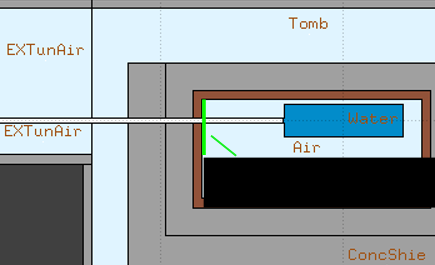
\includegraphics[height=0.5\textheight]{figures/Bird_view_BeamDump_Tomb.png}
\end{center}
\end{frame}

\begin{frame}{FLUKA simulation of the ILC Beam Dump}
\flukalogo
\begin{columns}
\begin{column}[c]{0.4\textwidth}
\includegraphics[height=0.45\textheight]{figures/FLUKA_quadrupole_model.png}\\
\small FLUKA simulation model of one of the ILC EXT lattice quadrupoles.
\end{column}
\begin{column}[c]{0.55\textwidth}
\begin{block}{Simulation step 2}
With Benno List (DESY): Python program to plug the real extraction line lattice into FLUKA.\\
Realistic simulation of the interaction between the neutrons and the lattice.
\end{block}
\begin{block}{Simulation step 3}
Simulating the neutrons reaching the interaction point in a full detector simulation.
\end{block}
\end{column}
\end{columns}
\vspace*{0.3cm}
\rule{12cm}{.1pt}
\begin{thebibliography}{9}
\setbeamertemplate{bibliography item}[text]
\bibitem{Smith} B. Smith (Rutherford Lab), \emph{Design drawings 0-TB-0067-300-00-A, 0-TB-0067-210-00-A, 0-TB-0067-404-00-A}, Dec. 2006 - Jan. 2007
\end{thebibliography}
\end{frame}
}

